\documentclass[9pt,english,utf8]{article}

\usepackage{amsmath}
\usepackage{amssymb}
\usepackage{amsfonts}
\usepackage{array}
\usepackage{booktabs}
\usepackage{caption}
\usepackage{cases}
\usepackage{enumerate}
\usepackage{graphicx}
\usepackage{subfigure}
\usepackage{units}
\usepackage{xcolor}
\usepackage{xspace}
\newcommand{\ignore}[1]{}
\newcommand{\remove}[1]{}


\graphicspath{{figures/}}


\title{Horizontal Gene Transfer Phylogenetics: A First Model-Based Approach\\
Simulation Experiments}
\begin{document}
\maketitle
%\tableofcontents

\section{Background}

In the main manuscript, we proposed an empirically derived estimator for the
\emph{synteny index} (SI) distance:

\begin{equation}
    \mathbb E[d_{SI}] = \left(1-\exp\left(-\frac{3-\frac{5k}{n-1}}{n} \lambda
    t\right)\right) \left(1-\frac{2k}{n-1}\right)
\end{equation}

In simulation experiments, we showed that this estimator performs well under
the studied model of \emph{horizontal gene transfer} (HGT). Here, we use the
inverse of the measure with the aim to derive additive distances:

\begin{equation}
    \hat d= \lambda t = -\frac{n}{3-\frac{5k}{n-1}}
    \log\left(1 - \frac{d_{SI}}{1-\frac{2k}{n-1}}\right)
\end{equation}

The goal of this experiment is to evaluate the SI distance in an applied
setting that is close to practice. Therefore, we simulate genome evolution of
multiple taxa that evolve under our HGT model as well as genome evolution with
single gene insertions and deletions. 

\paragraph{Genome evolution.} We used ALF~\cite{Dalquen:2012dx} as genome
evolution simulator of phylogenies with more than two taxa. ALF supports
various genome rearrangement operations, one of which being
\emph{translocations}. Translocations, more commonly known as
\emph{transpositions}, permute the gene order by moving blocks of genes from
one genomic location to another. ALF provides parameters to limit the number of
genes that are transposed in one event. In accordance with our model, we set
this number to 1. By doing so, ALF's genome rearrangement model under
transpositions is equivalent to the HGT model underlying our study.
Counterbalancing the computation time with a realistic scenario, the number of
genes per genome in the simulations is set to 1000. 

\medskip
The phylogenetic trees subject to reconstruction were sampled by ALF from the
tree of life. A random sample of nine trees is displayed in Figure
\ref{fig:mutations}(a). Many trees feature short internal edges
w.r.t.~external edges.  These configurations are known to be difficult to
reconstruct. To quantify the quality of reconstruction under various
evolutionary scenarios, we scaled these trees from small diameters (10 PAM) to
large (800 PAM) using a constant transposition rate of $0.001$. For each tree
size, 300 data samples (each encompassing a sampled tree, genes, gene order
sequences, etc.) were generated. 

\begin{figure}[tb]
    \subfigure[]{
    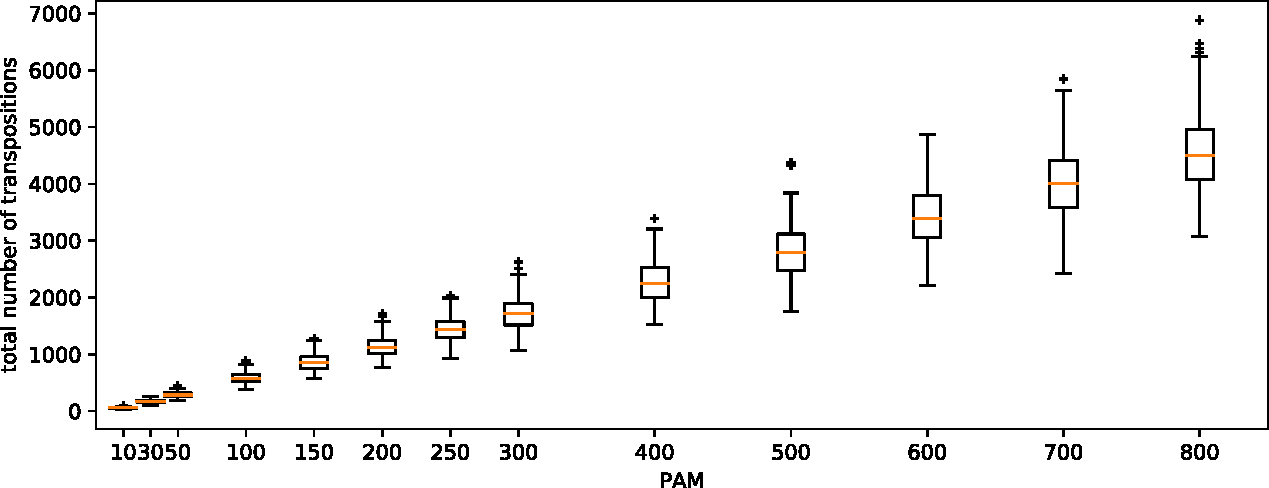
\includegraphics[width=0.60\columnwidth]{actual_mutations_s10_n10000}
    }
    \subfigure[]{
    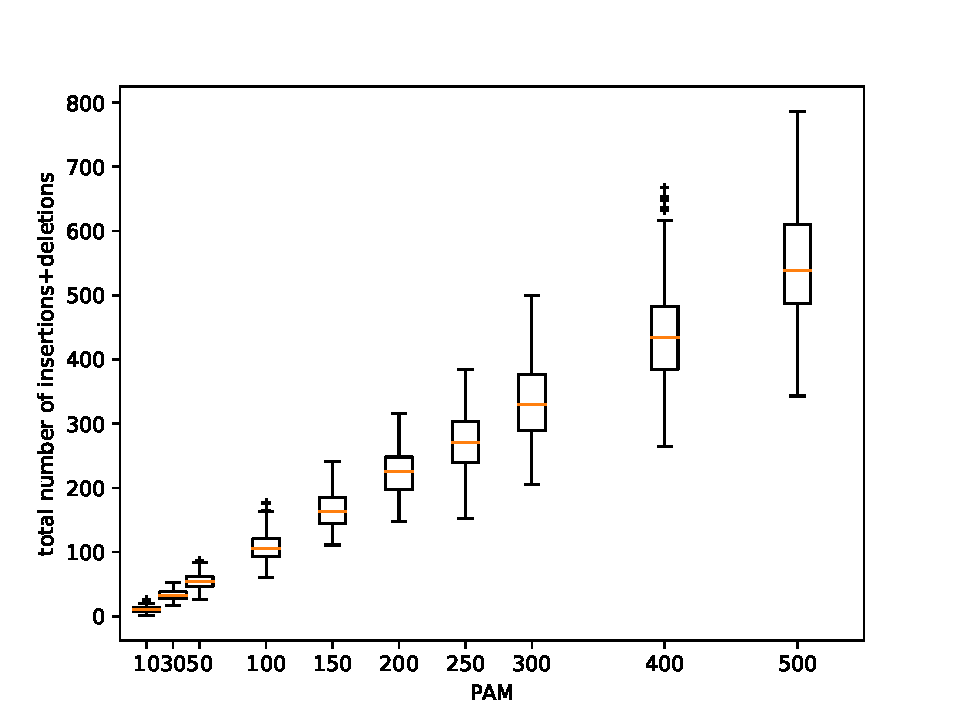
\includegraphics[width=0.35\columnwidth]{actual_mutations_s10_n10000_insertion_deletion}
    }
    \caption{\textbf{(a)} Total numbers of transpositions and \textbf{(b)}
    insertions+deletions per data point in the simulations.}
    \label{fig:mutations}
\end{figure}

In a subsequent experiment, we additionally simulated insertions and deletions
of individual genes, with an insertion/deletion rate of $0.0001$. Although ALF
does not support insertions of new genomic material in general, we exploited
ALF's functionality of simulating duplications with subsequent transposition.
ALF's data structures permit the distinction of orthologies between the
original gene and its duplicate. Thus, in our experiments, genes that emerged
as copies in duplication events are considered \emph{insertions}. The actual
numbers of insertions and deletions per PAM summarized over each tree is shown
in Figure~\ref{fig:mutations}(b).


\paragraph{Experimental setup.}
First, we performed a simple experiment in reconstructing pairwise distances,
i.e.  estimating the true evolutionary time from SI measures. To this end, we
sampled 10 genome sequences comprising 1000 genes per time point and calculated
$\hat d$ for different values of $k$.  

However, the main goal of this experiment is to assess the power of the SI
distance beyond the reconstruction of pairwise distances. That is, inferring
phylogenies comprising several taxa. The inverse SI being a \emph{distance}
measure we naturally followed standard procedure of distance-based
reconstruction. As tree reconstruction method, we chose \emph{Neighbor
Joining} (NJ), a classic and robust method for reconstructing unrooted trees.
The quality of the reconstruction is subsequently quantified by comparing the
topology of the reconstructed and the original tree using the classic
\emph{Robinson-Foulds} (RF) distance.  

\begin{figure}[tb]
    \centering 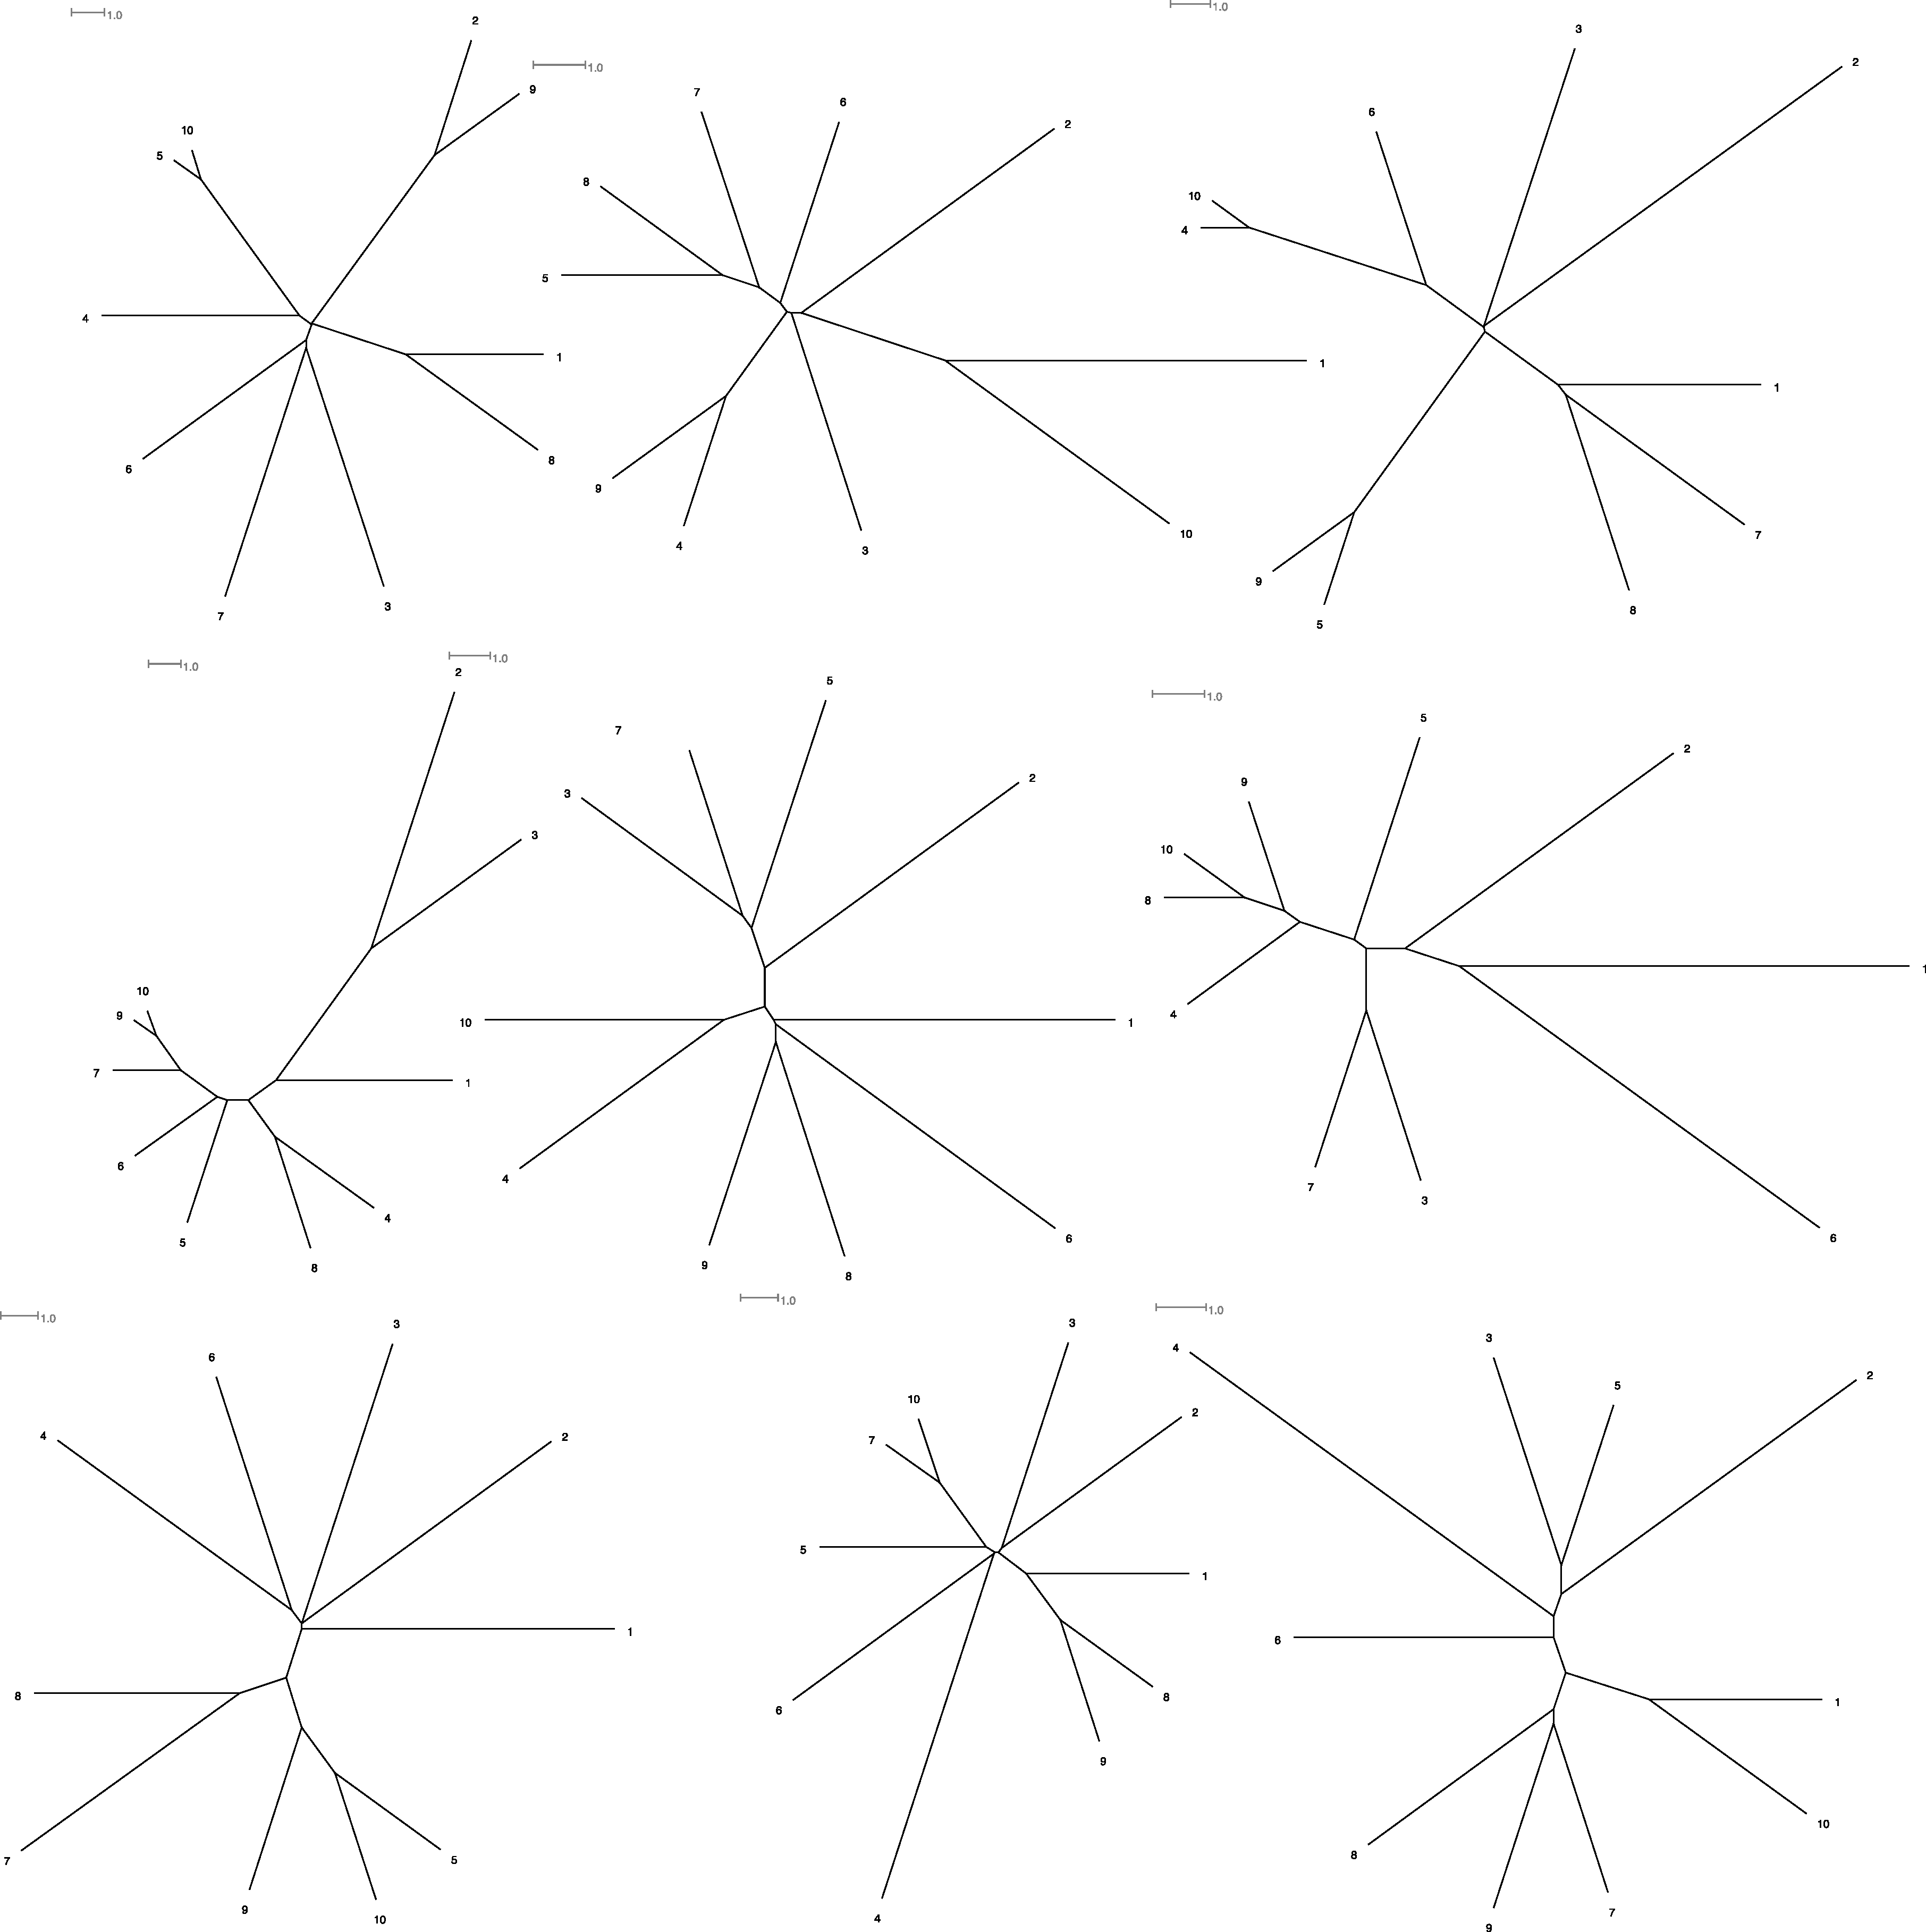
\includegraphics[width=\columnwidth]{true_trees_s10_pam10}

    \caption{A random sample of 9 phylogenetic trees of 10 taxa generated ALF
    and used in the simulation experiments.}
    \label{fig:tree}
\end{figure}

\paragraph{Results} The outcome of the experiment in pairwise distance
reconstruction is visualized in Figure~\ref{fig:results}(a). Despite the
inverted SI being not truthful to the true time, it remains additive for a
large range of evolutionary time. This indicates that the measure is
well-suited for distance-based reconstruction of phylogenetic trees. 

Figure~\ref{fig:results}(b) shows the outcome of the experiment of inferring
the 10 taxa comprising trees sampled from the tree of life (cf.
Figure~\ref{fig:tree}) from low to high numbers of mutations (measured in PAM).
The plot depicts well the two cases of poor reconstruction under the studied
HGT model: for low values of PAM, not enough HGTs are taking place, whereas for
large values of PAM, the gene order sequences are saturated from the excess of
HGT events. 

\begin{figure}[tb]
\begin{center}

\begin{tabular}{cc}
\hspace{-3.5cm}
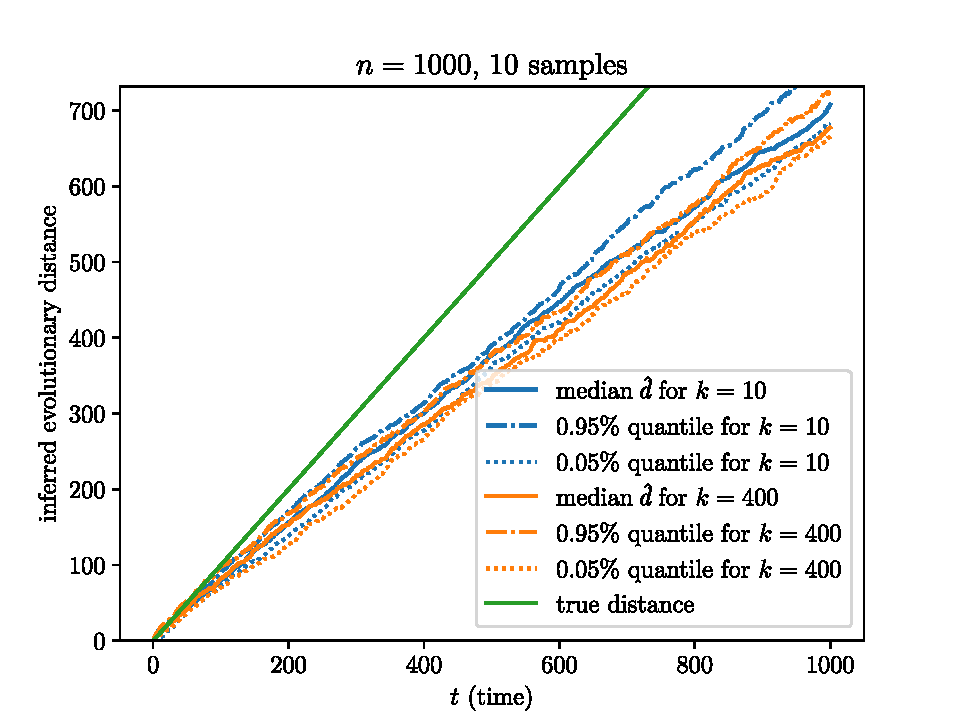
\includegraphics[width = 3.7in,angle=0]{distance_plot_n1000_s10_inv}
&
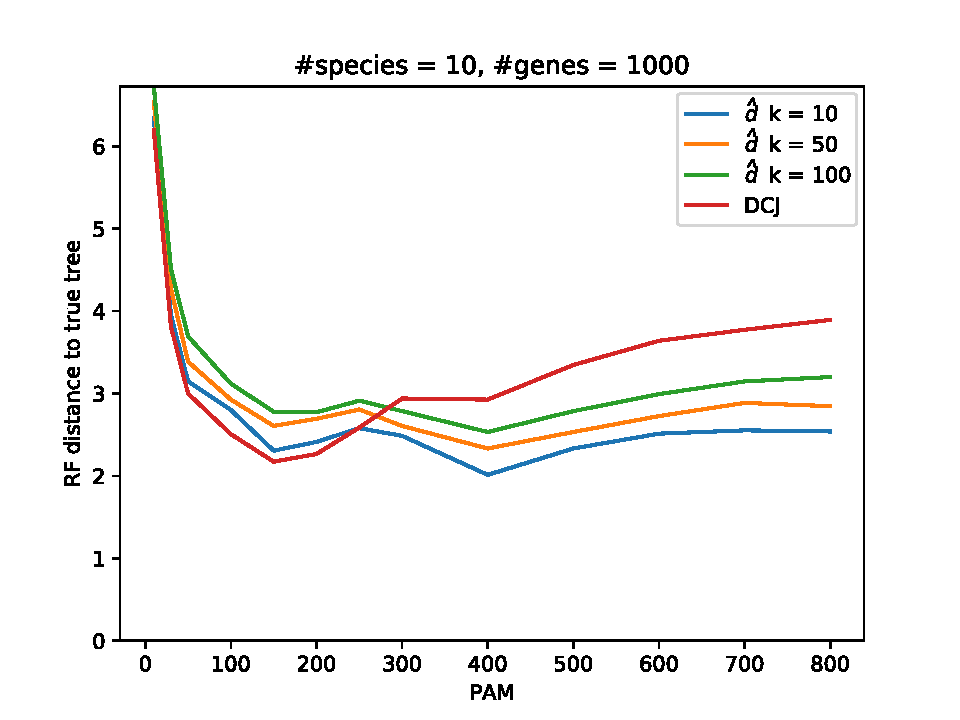
\includegraphics[width = 3.7in,angle=0]{boxplot_s10_n1000} \\
% \hspace{-2.5in}
\hspace{-3.5cm}
 (a) & %\hspace{-3in} 
 (b) 
\end{tabular}

   \caption{\textbf{(a)} Median, $5\%$-, and $95\%$-quantiles of inferred
    pairwise distances $\hat t = d_{SI}$ for $k=10, 400$. \textbf{(b)} Mean RF
distances between the reconstructed and true trees of the simulation. }
\label{fig:results}
\end{center}
\end{figure}

\remove
{
\begin{figure}[tb]
    
    \subfigure[]{
    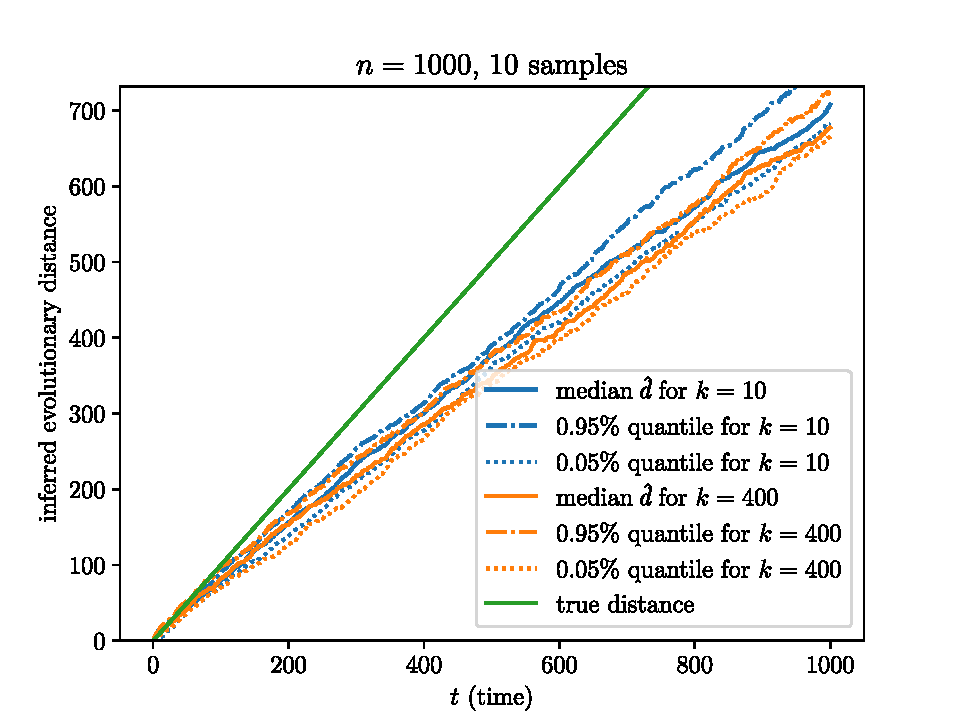
\includegraphics[width=0.8\columnwidth]{distance_plot_n1000_s10_inv}
    }
    \subfigure[]{
    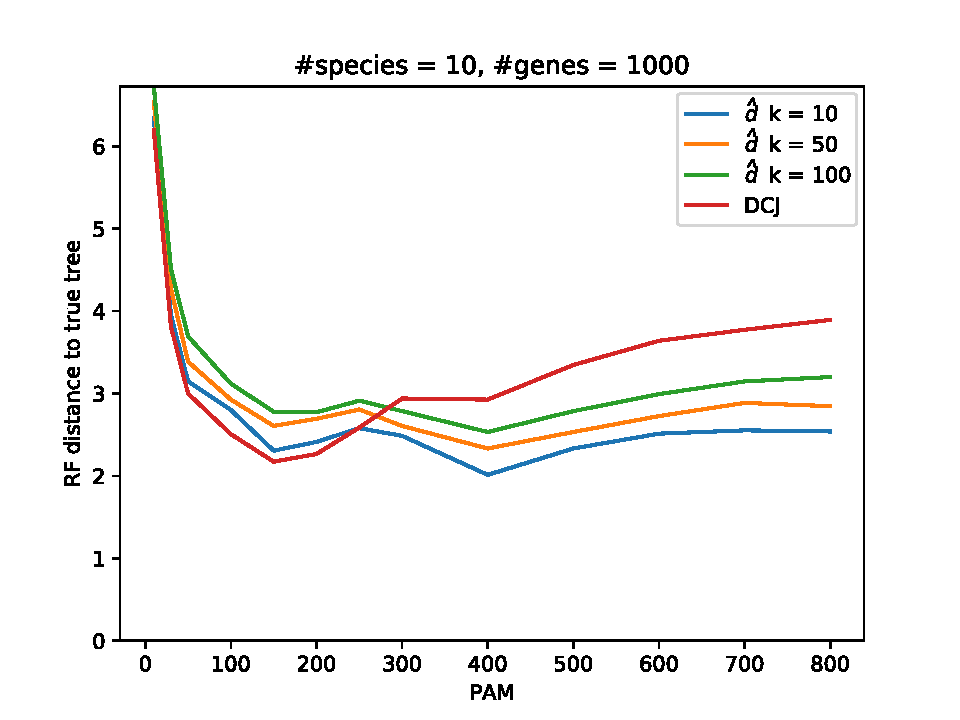
\includegraphics[width=0.8\columnwidth]{boxplot_s10_n1000}
    }

    \caption{\textbf{(a)} Median, $5\%$-, and $95\%$-quantiles of inferred
    pairwise distances $\hat t = d_{SI}$ for $k=10, 400$. \textbf{(b)} Mean RF
distances between the reconstructed and true trees of the simulation. }
\label{fig:results}
\end{figure}
}

Next to the SI distance, we included the double-cut-and-join (DCJ)
distance~\cite{Yancopoulos:2005bm,Bergeron:2006uj} for comparison. The DCJ
distance is parsimonious (i.e., non-additive) and the most prevalent measure
used for quantifying genome rearrangement, including transpositions. Under our
model of HGT, the DCJ distance is not exact, but only an approximation of the
true parsimonious distance. To the best of our knowledge,
GRAPPA-TP~\cite{Yue:2008ima} and DERANGE 2~\cite{Blanchette:1996wx} are the
only implementation that aim to compute the \emph{transposition distance}.
DERANGE 2 implements an exhaustive method with exponential runtime in the
comparison of genome sequences that are separated by many transpositions and
therefore is not suited for the purposes of this experiment. We were not able
to include GRAPPA-TP into our experimental framework, because of its unstable
behavior, terminating prematurely in many of the pairwise comparisons.

In our experiment the DCJ distance outperformed SI for low PAM, where
transpositions rarely overlap and therefore breakpoint reuse does not often
occur. However, with rising PAM, these events become more prevalent, violating
the presumed law of parsimony.  The SI distance, maintaining additivity,
outperforms the DCJ distance eventually---even under poor choices of $k$ (cf.
$k=100$).

\medskip
The last experiment concerns the impact of gene content changes, i.e.
insertions and deletions of individual genes, on the SI distance. Unlike DCJ,
which requires that that each gene occurs exactly once in all compared genomes,
the SI distance is able to handle such gene content modifications.  Here, we
compare our estimator of the true evolutionary time $\hat d$ to the
\emph{Jaccard distance} over the gene content of the two compared sequences.
This distance is equivalent to $d_{SI}$ for $k \geq \frac{n}{2}$, where $n$ is
the length of the largest sequence over all pairwise comparisons. In our
experiment, we refer to this measure as the \emph{gene content} distance
$d_{GC}$. Figure~\ref{fig:results_indel} shows the outcome of the corresponding
experiment described in above with insertion/deletion rate of $0.0001$. Since
the number of such events in the simulated trees is about five times lower than
the number of transpositions (cf.~Figures~\ref{fig:mutations}(a) and (b)), the
gene content distance remains additive over all values of PAM, but at the same
time it suffers from the rare occurrences of changes in gene content. The
inability to separate taxa in the reconstructed phylogenetic tree leads results
in the poor performance of the gene content distance for phylogenies with span
lower than 400 PAM. The inverted SI distance $\hat d$ perform continuously
well, in particular for low values of $k$. 


\begin{figure}[tb]
    
    \centering 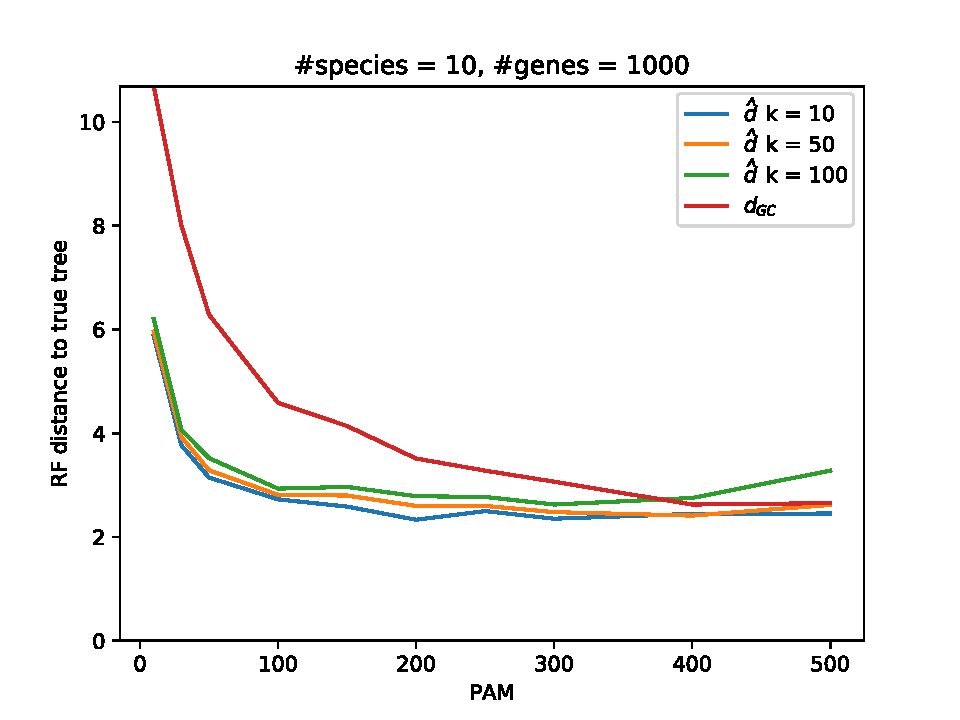
\includegraphics[width=0.8\columnwidth]{boxplot_s10_n1000_indel}

    \caption{Mean RF distances between the reconstructed and true trees of the
    genome evolution experiment with insertions and deletions.}
\label{fig:results_indel}
\end{figure}


\bibliographystyle{plain} 
\bibliography{references} 

\end{document}
